\bookmarksetup{startatroot}
\thispagestyle{empty}
\chapter*{Caderno de imagens}
\addcontentsline{toc}{chapter}{\textcolor{ocre}{Caderno de imagens}}

\begin{figure}[h]
\includegraphics[width=\textwidth]{figura_3.1}
\caption{\textit{Primavera}, de Sandro Botticelli. 1482}
\label{fig:mesh3.1}
\end{figure}

Algum texto aqui.

\newpage

\begin{figure}[h]
\includegraphics[width=\textwidth]{figura_3.2}
\caption{\textit{O nascimento de Vênus}, de Sandro Botticelli. 1483}
\label{fig:mesh3.2}
\end{figure}

Há uma correção anatômica dos corpos, e grande preocupação com as noções de profundidade, volume (em especial, por meio da iluminação), proporção e perspectiva. O ponto de fuga do quadro está situado entre a fase e os seios de Vênus. Trata-se de um tema clássico, retirado da tradição literária grega presente na teogonia. A concha figura como símbolo para o feminino (abertura em referência à mucosa vaginal), em especial pelo que Vênus (Afrodite) representa.

\newpage

\begin{figure}[h]
\includegraphics[width=\textwidth]{figura_3.3}
\caption{\textit{Davi}, de Michelangelo Buonarroti. 1501-1504}
\label{fig:mesh3.3}
\end{figure}

Algum texto aqui.

\newpage

\begin{figure}[h]
\includegraphics[width=\textwidth]{figura_3.4}
\caption{\textit{Vênus de Urbino}, de Ticiano. 1538}
\label{fig:mesh3.4}
\end{figure}

Algum texto aqui.

\newpage

\begin{figure}[h]
\includegraphics[width=\textwidth]{figura_5.1}
\caption{\textit{A última ceia}, de Leonardo da Vinci. 1495-1498}
\label{fig:mesh5.1}
\end{figure}

Do Renascimento, note a presença de tons harmoniosos e grande preocupação com a geometria, equilíbrio e simetria da obra. Há um destaque para a claridade solar e para a suavização das cores.

\newpage

\begin{figure}[h]
\includegraphics[width=\textwidth]{figura_5.2}
\caption{\textit{A última ceia}, de Jacopo Tintoretto. 1592-1594}
\label{fig:mesh5.2}
\end{figure}

Em comparação com o quadro anterior, note a visão diagonal, que transmite maior sensação de profundidade. Perceba também o contraste de cores e entre a luz e a sombra. Veja que a figura de Jesus não ocupa o centro da obra (ponto de fuga). A pintura, ainda assim, é mais dinâmica e vívida, alinhando-se mais com a realidade. Também é relevante o percurso em ``U'', o qual requer a exploração visual da obra — de maior grau de complexidade.

\newpage

\begin{figure}[h]
\includegraphics[width=\textwidth]{figura_5.3}
\caption{\textit{A ceia em Emaús}, de Caravaggio. 1601}
\label{fig:mesh5.3}
\end{figure}

Os movimentos e feições indicam grande expressividade.

\newpage

\begin{figure}[h]
\includegraphics[width=\textwidth]{figura_5.4}
\caption{\textit{A incredulidade de São Tomé}, de Caravaggio. 1601-1602}
\label{fig:mesh5.4}
\end{figure}

Note a utilização de um jogo de luz e sombra. Com a feição oculta, há um enfoque na carne de Jesus.

\newpage

\begin{figure}[h]
\includegraphics[width=\textwidth]{figura_5.5}
\caption{\textit{Morte da virgem}, de Caravaggio. 1604-1606, 1602}
\label{fig:mesh5.5}
\end{figure}

Veja como a morte de Maria é representada de maneira não tão serena como de costume. Há a utilização de vestimentas vermelhas, e a feição da mulher é expressa inchada e amarelada.

\newpage

\begin{figure}[h]
\includegraphics[width=\textwidth]{figura_5.6}
\caption{\textit{O rapto de Proserpina}, de Gian Lorenzo Bernini. 1621-1622}
\label{fig:mesh5.6}
\end{figure}

Na mitologia grega, Perséfone é a deusa da natureza, filha de Zeus e Deméter (deusa da colheita e fertilidade). Fora raptada por Hades (Plutão) e levada ao submundo. Para solucionar o impasse, Zeus ordenara que a filha passasse parte do ano no mundo dos mortos (correspondente à estação de inverno), e parte do ano junto da mãe (correspondente à estação da primavera) até o verão, quando deveria retornar (outono) — explicação para a ocorrência das estações do ano. É necessário, novamente, destacar a expressividade e dramaticidade presentes na obra, e a busca por carnalidade por meio do realismo (veja os detalhes na pele da deusa, cuja coxa é pressionada por Plutão).

\newpage

\begin{figure}[h]
\includegraphics[width=\textwidth]{figura_5.7}
\caption{\textit{O êxtase de Santa Teresa}, de Gian Lorenzo Bernini. 1647-1652}
\label{fig:mesh5.7}
\end{figure}

Santa Teresa possuía frequentes visões que registrava em seu diário. Há um destaque para a dicotomia entre a lança do prazer e do sofrimento, e o êxtase em questão representa também uma forma de sensualização.

\newpage

\begin{figure}[h]
\includegraphics[width=\textwidth]{figura_5.8}
\caption{\textit{Beata Ludovica Albertoni}, de Gian Lorenzo Bernini. 1671-1674}
\label{fig:mesh5.8}
\end{figure}

De maneira semelhante à escultura anterior, há um processo de sensualização.

\newpage

\begin{figure}[h]
\includegraphics[width=\textwidth]{figura_5.9}
\caption{\textit{As três graças}, de Peter Paul Rubens. 1630-1635}
\label{fig:mesh5.9}
\end{figure}

Compare a obra com a representação das três graças em \textit{Primavera}, de Botticelli, e note o maior enfoque na carnalidade e nas expressões faciais das mulheres.

\newpage

\begin{figure}[h]
\includegraphics[width=\textwidth]{figura_5.10}
\caption{\textit{O enterro do Conde Orgaz}, de El Greco. 1587}
\label{fig:mesh5.10}
\end{figure}

Note a relação com a passagem bíblica de Pedro e as chaves do céu, refletida na presença de santos e anjos, imersos em um quadro saturado (dinâmico), com muitas informações visuais apresentadas em um eixo ascensional. Note a arte mundana e os temas projetados.

\newpage

\begin{figure}[h]
\includegraphics[width=\textwidth]{figura_5.11}
\caption{\textit{A apoteose de Santo Inácio}, de Andrea Pozzo. 1691-1694}
\label{fig:mesh5.11}
\end{figure}

A obra utiliza-se diretamente da noção de três dimensões e busca causar a sensação de ascendência do espectador.

\newpage

\begin{figure}[h]
\includegraphics[width=\textwidth]{figura_5.12}
\caption{Santuário do Bom Jesus do Monte, em Portugal.}
\label{fig:mesh5.12}
\end{figure}

A arquitetura barroca, de maneira geral, era elaborada e intrincada. É interessante notar, no caso da fotografia acima, a forma pela qual as escadarias construídas em zigue-zague atuam como desvios para a salvação do indivíduo.

\newpage

\begin{figure}[h]
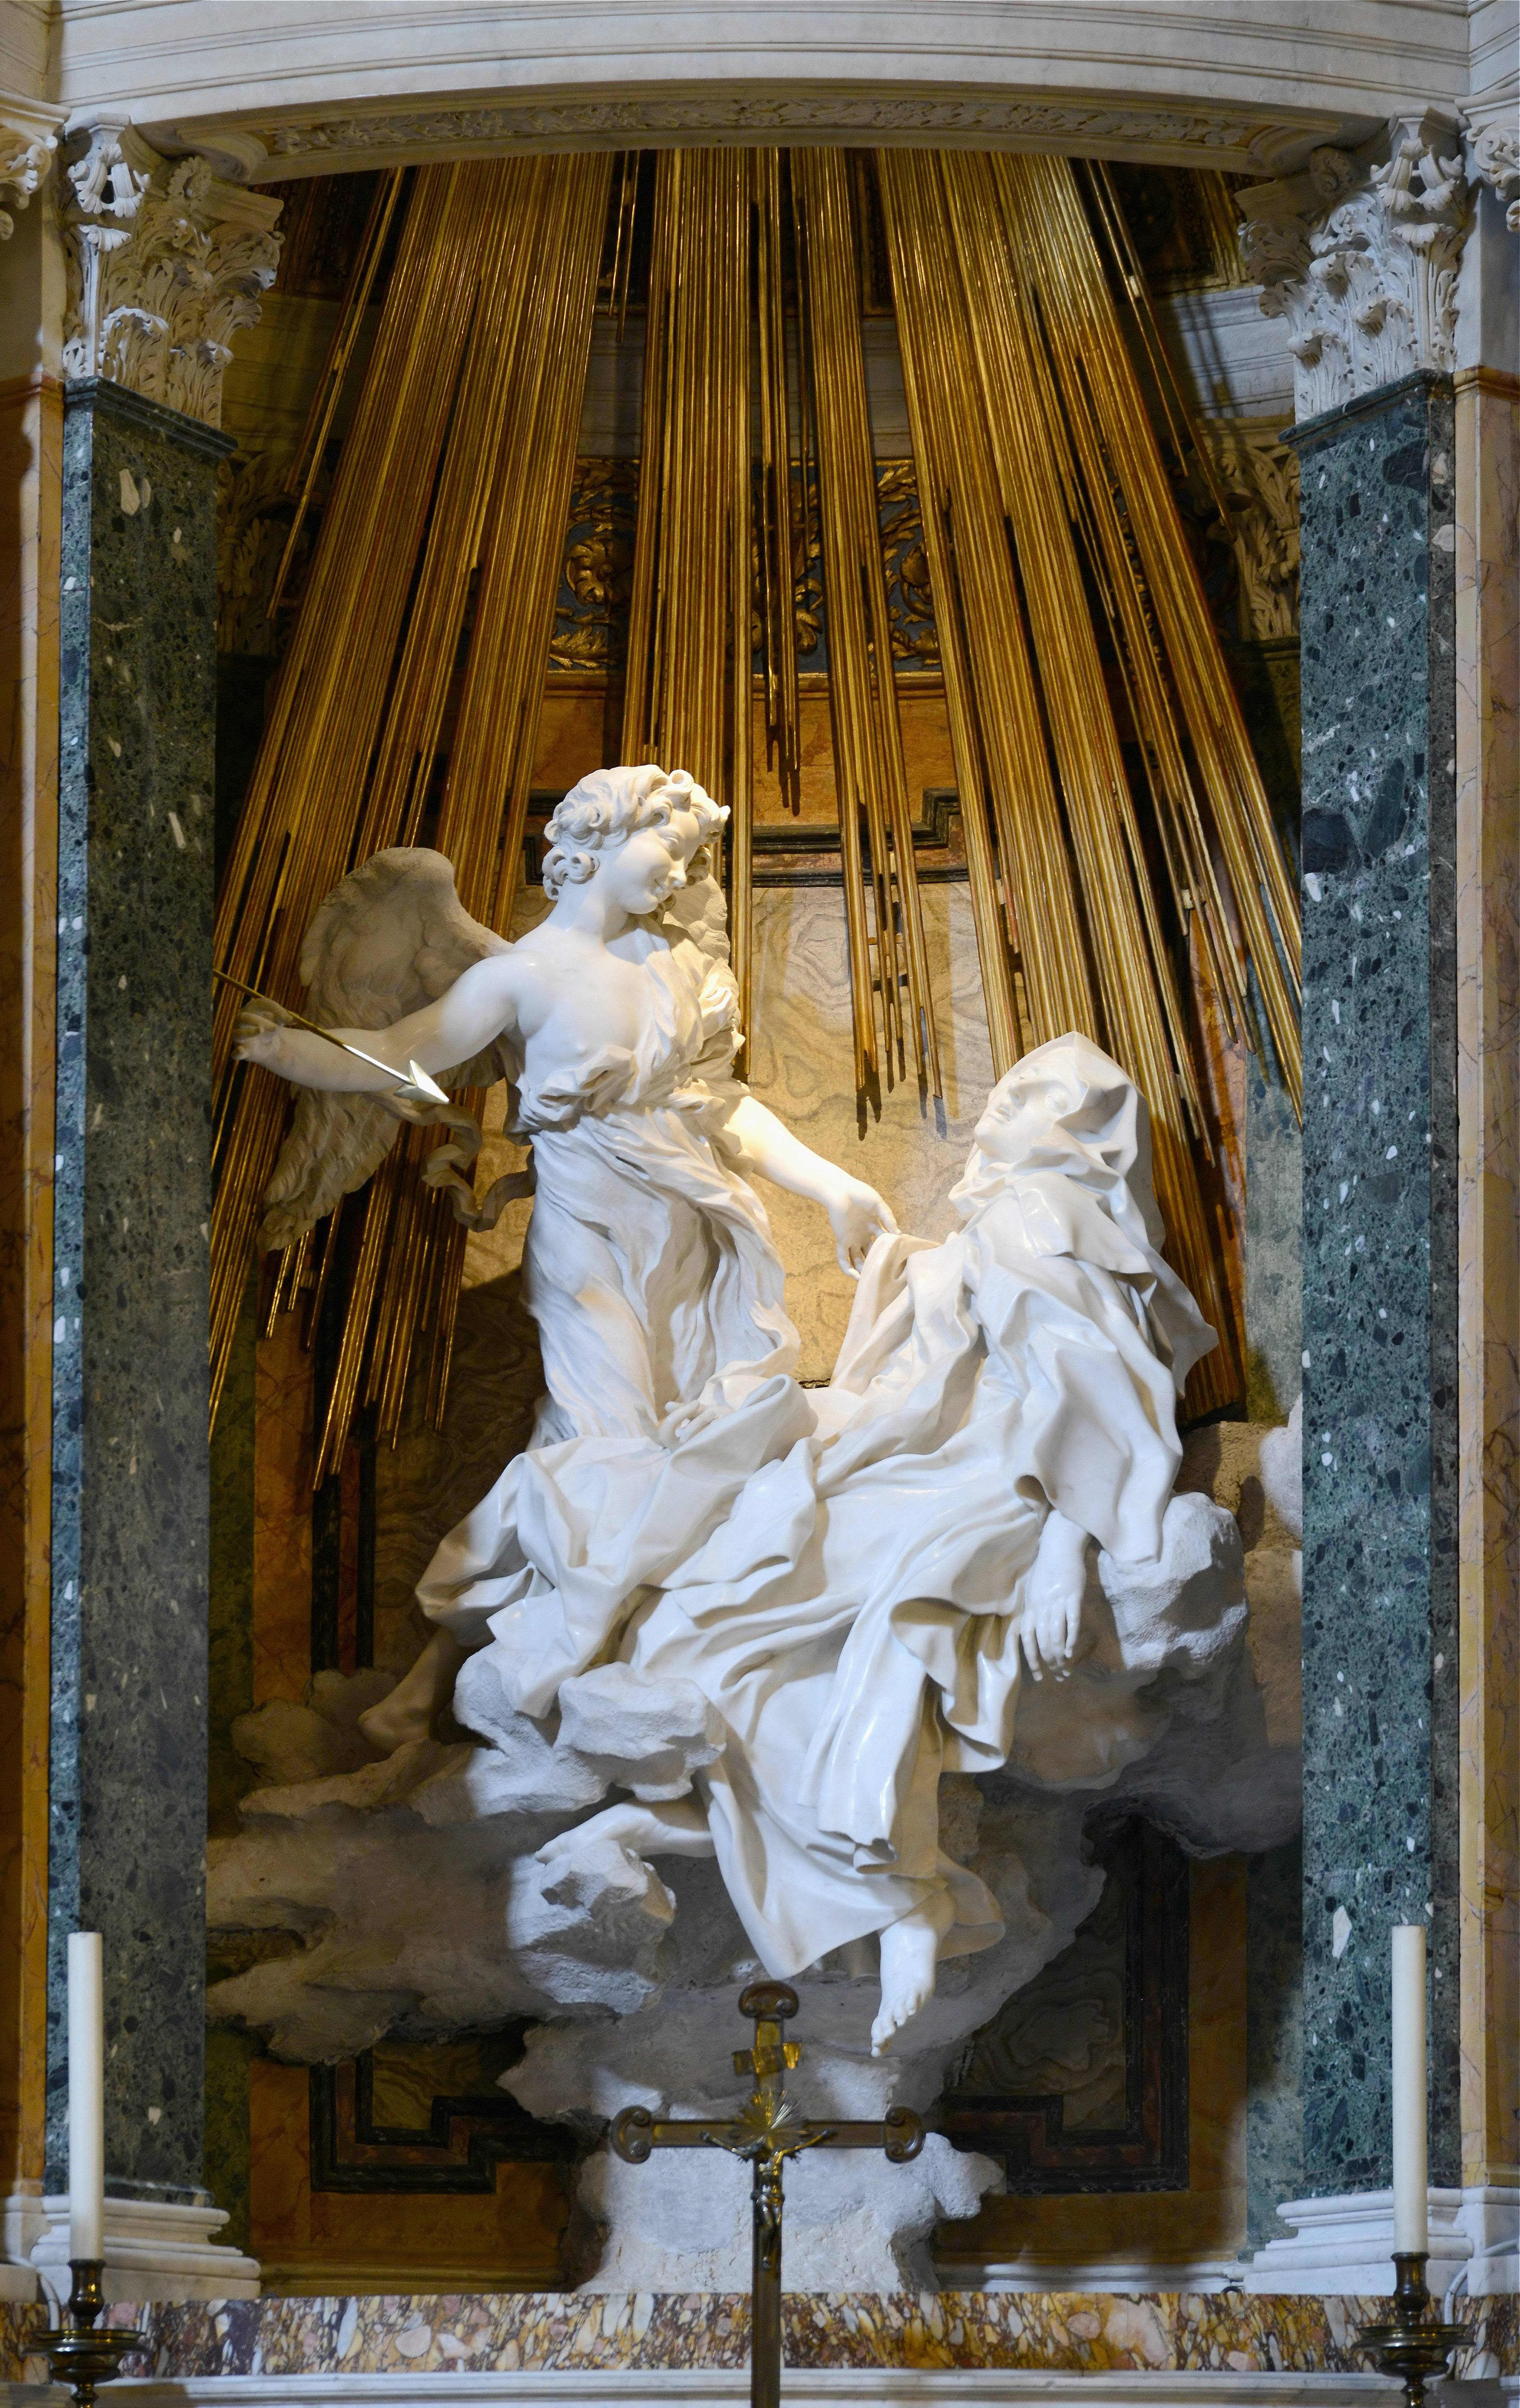
\includegraphics[width=\textwidth]{figura_9.1}
\caption{Rio Tejo}
\label{fig:mesh9.1}
\end{figure}

\newpage

\begin{figure}[h]
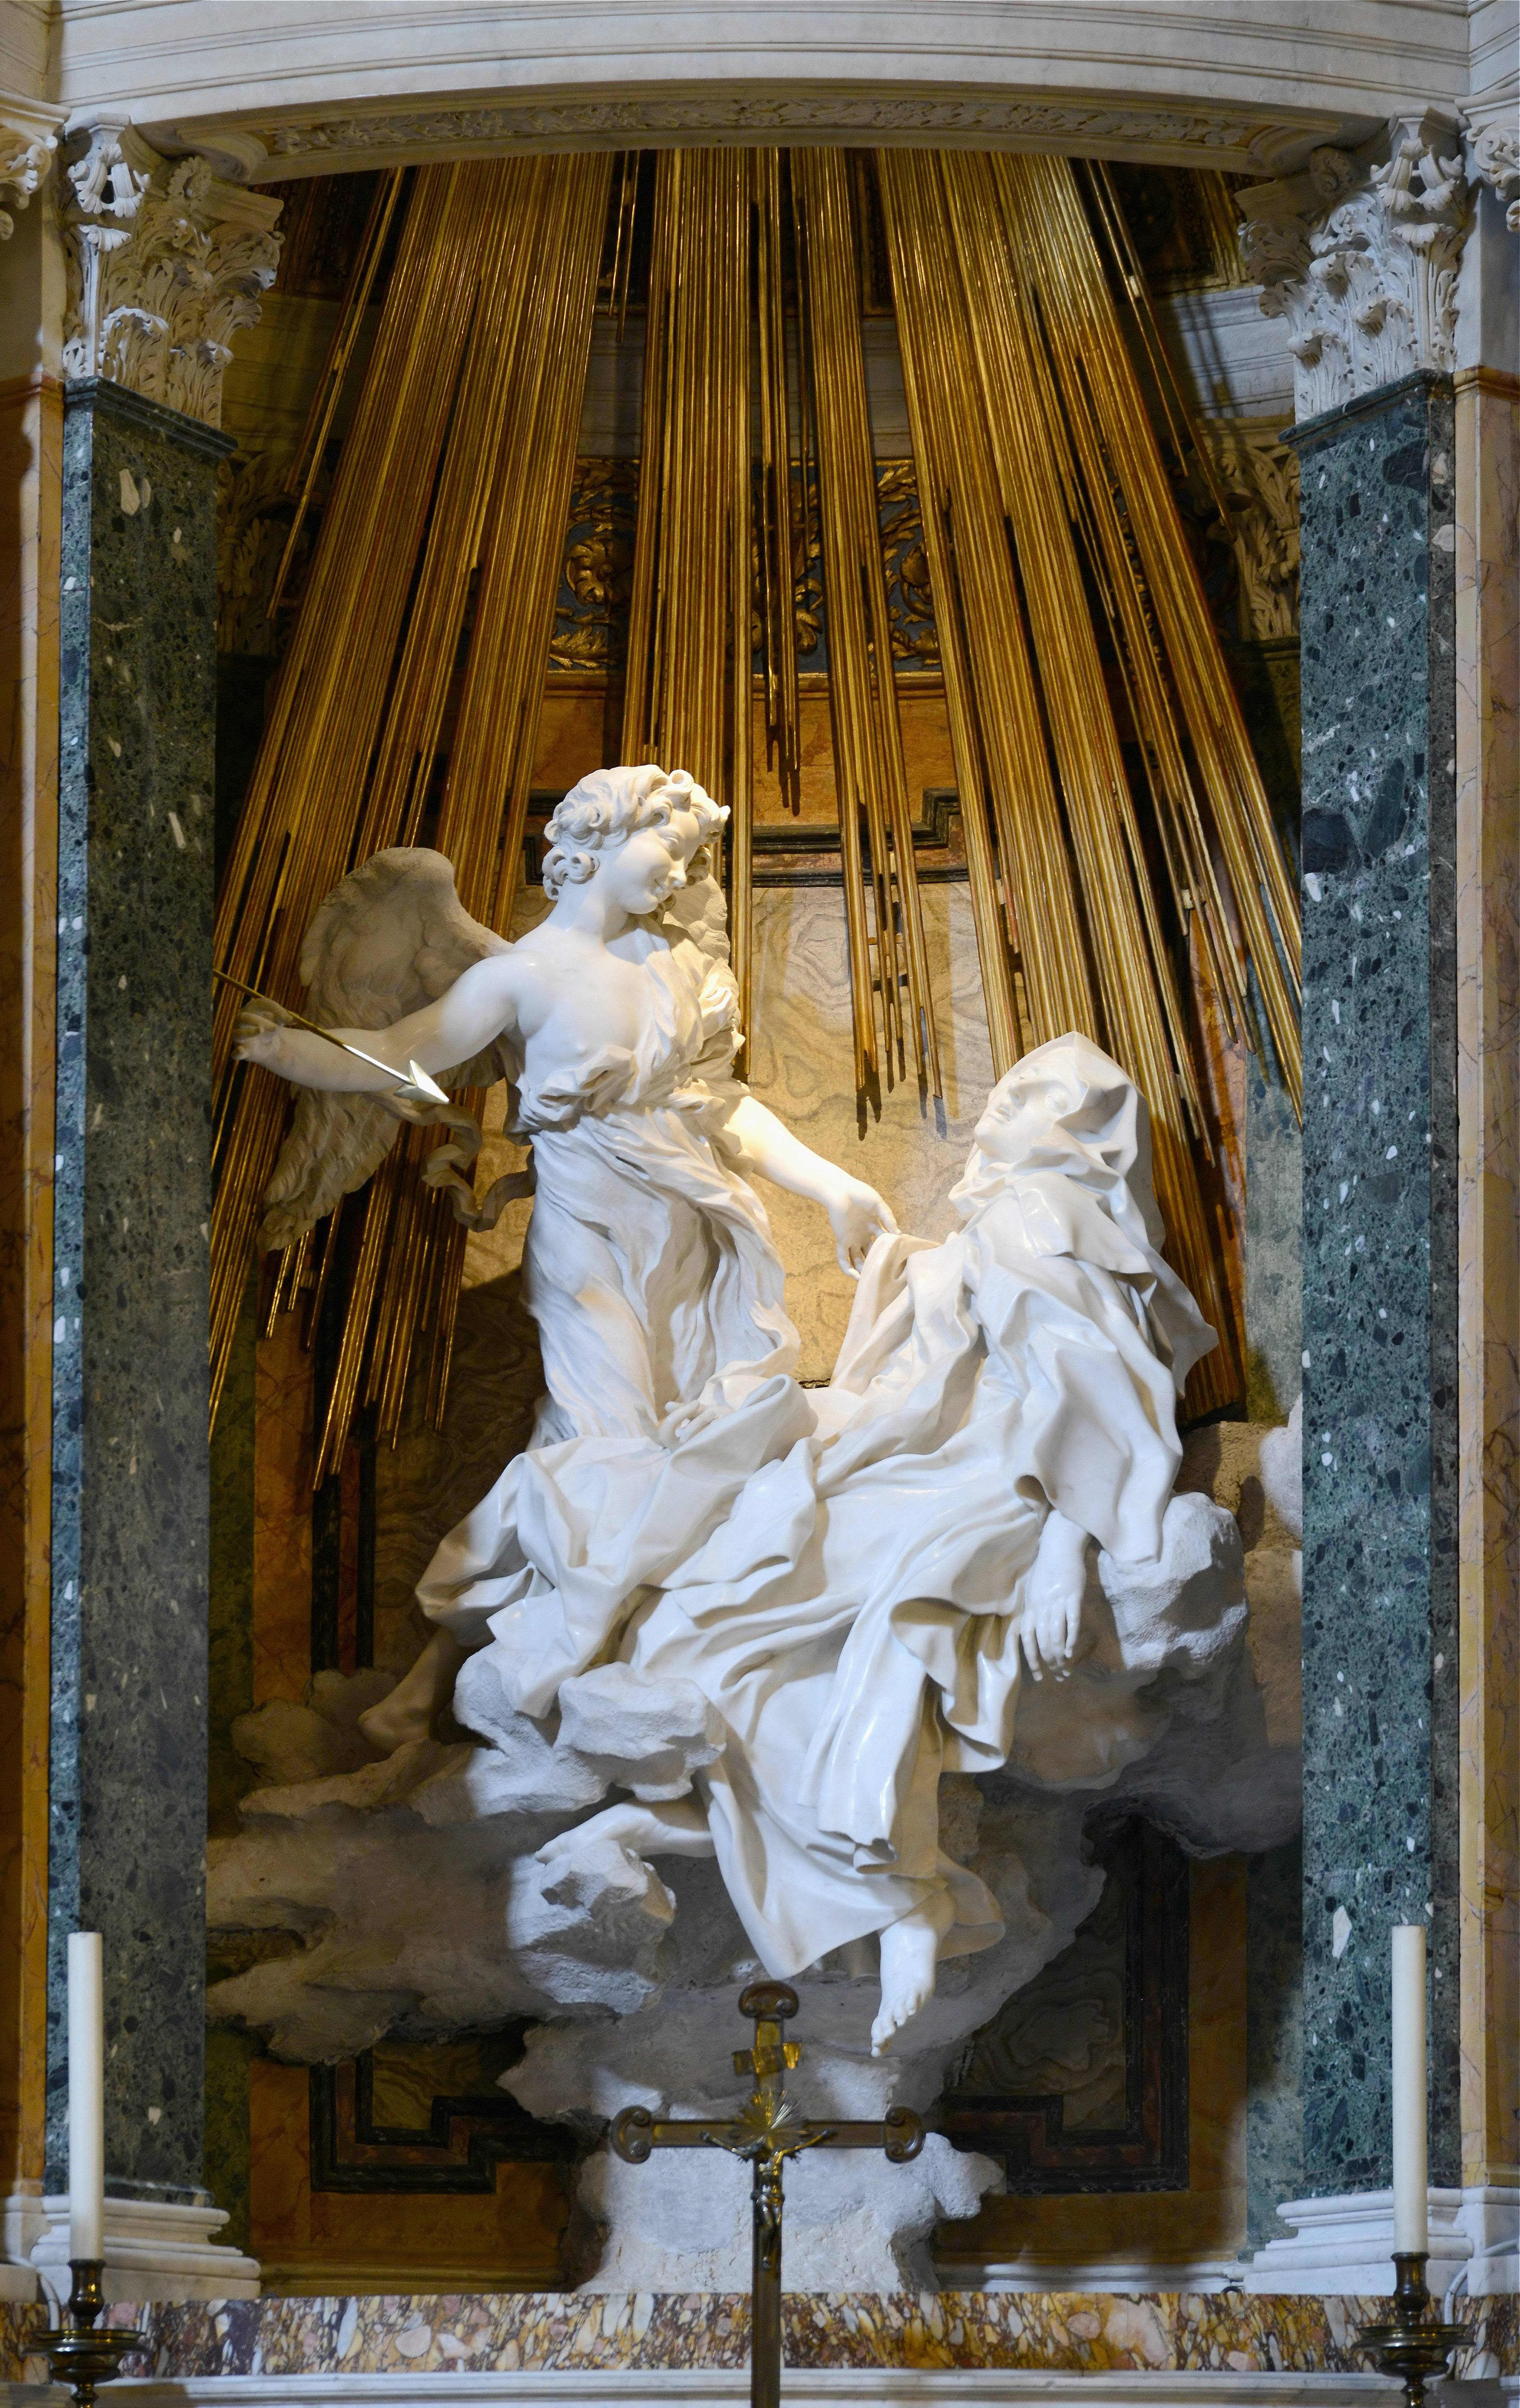
\includegraphics[width=\textwidth]{figura_9.2}
\caption{Ribeirão do Carmo}
\label{fig:mesh9.2}
\end{figure}

\newpage

\begin{figure}[h]
\includegraphics[width=\textwidth]{figura_10.1}
\caption{\textit{A Liberdade guiando o povo}, de Eugène Delacroix. 1830}
\label{fig:mesh10.1}
\end{figure}

Note que a figura da Liberdade utiliza um barrete frígio, que representa a república (também a forma como a questão reformista aparecia nas artes plásticas).

\newpage

\begin{figure}[h]
\includegraphics[width=\textwidth]{figura_22.1}
\caption{\textit{A redenção de Cam}, de Modesto Brocos. 1895}
\label{fig:mesh22.1}
\end{figure}

No contexto do Naturalismo no Brasil, o quadro exemplifica de maneira clara a ideia de apuração do sangue. Sob o viés cientificista da época, as mulheres negras teriam um instinto em se relacionar com homens brancos — melhor patrimônio genético, como um macho de raça superior. No contexto brasileiro, buscava-se a maior branquitude possível da população.

\newpage

\begin{figure}[h]
\includegraphics[width=\textwidth]{figura_28.1}
\caption{\textit{Les Demoiselles d'Avignon}, de Pablo Picasso. 1907}
\label{fig:mesh28.1}
\end{figure}

Algum texto aqui.

\newpage

\begin{figure}[h]
\includegraphics[width=\textwidth]{figura_28.2}
\caption{\textit{Frineia em frente ao Areóago}, de Jean-Léon Gerôme. 1861}
\label{fig:mesh28.2}
\end{figure}

Obra contemporânea que retrata o episódio do julgamento de Frineia. Assim como em \textit{O nascimento de Vênus}, os braços levantados possibilitam maior destaque na representação dos seis.

\newpage

\begin{figure}[h]
\includegraphics[width=\textwidth]{figura_28.3}
\caption{\textit{Olympia}, de Édouard Manet. 1863}
\label{fig:mesh28.3}
\end{figure}

Algum texto aqui.

\newpage

\begin{figure}[h]
\includegraphics[width=\textwidth]{figura_28.4}
\caption{\textit{L'Origine du monde}, de Gustave Courbet. 1866}
\label{fig:mesh28.4}
\end{figure}

\newpage

\begin{figure}[h]
\includegraphics[width=\textwidth]{figura_28.5}
\caption{\textit{Retrato da mãe do artista}, de Pablo Picasso. 1896}
\label{fig:mesh28.5}
\end{figure}

Algum texto aqui.

\newpage

\begin{figure}[h]
\includegraphics[width=\textwidth]{figura_28.6}
\caption{\textit{Campo de trigo com corvos}, de Vincent van Gogh. 1890}
\label{fig:mesh28.6}
\end{figure}

Algum texto aqui.

\newpage

\begin{figure}[h]
\includegraphics[width=\textwidth]{figura_28.7}
\caption{\textit{Mont Sainte-Victoire}, de Paul Cézanne. 1904-1906}
\label{fig:mesh28.7}
\end{figure}

Algum texto aqui.

\newpage

\begin{figure}[h]
\includegraphics[width=\textwidth]{figura_28.8}
\caption{\textit{San Giorgio Maggiore au crépuscule'}, de Claude Monet. 1908}
\label{fig:mesh28.8}
\end{figure}

Algum texto aqui.

\newpage

\begin{figure}[h]
\includegraphics[width=\textwidth]{figura_28.9}
\caption{\textit{O grito}, de Edvard Munch. 1893}
\label{fig:mesh28.9}
\end{figure}

Algum texto aqui.

\newpage

\begin{figure}[h]
\includegraphics[width=\textwidth]{figura_28.10}
\caption{\textit{Sick transit}, de José Paulo Paes. 1973}
\label{fig:mesh28.10}
\end{figure}

Algum texto aqui.

\newpage

\begin{figure}[h]
\includegraphics[width=\textwidth]{figura_28.11}
\caption{\textit{Fonte}, de Marcel Duchamp. 1917}
\label{fig:mesh28.11}
\end{figure}

Algum texto aqui.